
\chapter{尤度比を使ったモデルとデータの比較}
モデル$M$において得られるデータ元に、母数を最尤推定する。新たに作られた最尤モデル上での尤度と元のモデル$M$での尤度の比がある分布に従うことがわかっている。
このことを利用して、もともモデル$M$でデータを予測してもいいのかを考察する。

\section{尤度比検定}
母数の個数が$k$個のモデル$M(\theta)$とする($\theta$は$k$次元ベクトル)。
モデル$M(\theta)$からサンプリングしたサンプルサイズ$n$の標本$x=(x_1,x_2,\cdots,x_n)$を得たとする。
この標本$X$から$\theta$のうち$r$個の母数に関する最尤推定量を$\bar{\theta}$得たとする。
$\bar{\theta}$のうち$k-r$個はモデル由来の母数であり、$r$個は標本から推定した母数である。
このことから、$\bar{\theta}$は自由度$r$の母数のベクトルと言う。

もとのモデル$M(\theta)$における標本$X$に対する尤度は、$L(\theta,x)$とする。
また、最尤モデル$M(\bar{\theta})$での尤度は、$L(\bar{\theta},x)$とする。
このとき、これら尤度の比がカイ二乗分布分布に従うことがわかっている\footnote{ただしいくらかの条件がある}。
つまり、
\begin{equation*}
    -2\log\lambda(X)\sim \chi^2_{k-r}
\end{equation*}
ただし、
\begin{equation*}
    \lambda(X) = \frac{L(\theta,x)}{L(\bar{\theta},x)} 
\end{equation*}
である。

\section{正規モデルにおける尤度比検定}

$\sigma^2_0$を設定した正規モデル$M(\mu_0;\sigma^2_0)$について考察する。
この正規モデルからサンプリングを行なった標本$X$とする。
標本から得た最尤正規モデルを$M(\bar{x};\sigma^2_0)$とする。
それぞれのモデル内での標本$X$の尤度を$L(\mu_0,X),L(\bar{x},X)$とする。
具体的な数式は、
\begin{align}
    L(\mu_0,X)=\frac{1}{\sqrt{2\pi\sigma^2}}\exp(-\frac{\sum(x_i-\mu_0)}{2\sigma^2})\\
    L(\bar{X},X)=\frac{1}{\sqrt{2\pi\sigma^2}}\exp(-\frac{\sum(x_i-\bar{X})}{2\sigma^2})\\
\end{align}
これらから$\lambda(X)$を計算すると、
\begin{align}
    -2\log\lambda(X) &= -2(-\frac{n}{2\sigma^2_0}(\bar{x}-\mu_0)^2) \\
    &= \frac{n}{\sigma^2_0}(\bar{x}-\mu_0)^2 \sim \chi^2_1 \\
\end{align}
である。

\subsubsection{数値実験}
モデルと同じ確率密度関数からサンプリングを行い、尤度比検定を行なってみる。

数値実験を行なってみる。具体的に、正規分布$N(170,5.8^2)$からサンプリングした標本1000個を集める。
標本から平均値を求め、これを最尤推定量とする(xbar)。
この最尤モデル$M(\mu;\sigma^2=5.8^2) $における標本の尤度を計算する(loglike2)。
同様に、モデル$M(170;\sigma^2=5.8^2)$における標本の尤度を計算する(loglike)。
以上から尤度比を計算し、それが$\chi^2_1$分布と一致することを確かめる。
以下がコードである。

\begin{lstlisting}
norm_ = norm(170,5.8)
data_ = norm.rvs(170,5.8,size=(1000,10))
xbar = np.average(data_,axis=1)
loglike_ = np.prod(norm_.pdf(data_),axis=1)
#loglike2_ = np.prod(norm(xbar,5.8).pdf(data_),axis=0)
#print(np.prod(norm(xbar,5.8).pdf(data_),axis=1),xbar)

loglike2_ = []
for item in data_:
    #print(item.shape)
    a = norm(np.average(item),5.8).pdf(item)
    loglike2_.append(np.prod(a))

y = -2*np.log(loglike_/loglike2_)
x = sorted(y)
y_ = np.arange(len(y))/len(x)
plt.plot(x,y_)
plt.plot(x,chi2.cdf(x,df=1))
plt.show()

\end{lstlisting}

$N(170,5.8^2)$と$N(175,5.8^2)$と言う2種類の密度関数からサンプリングを行いそれぞれ結果を図\ref{fig:loglikelihood_test_simulation_norm}(a)および(b)に示す。
図\ref{fig:loglikelihood_test_simulation_norm}(a)は、モデルとデータの分布が一致していることから、累積分布が$\chi^2_1$の累積分布にかなり近いことがわかる。
図\ref{fig:loglikelihood_test_simulation_norm}(b)は、モデルとデータが一致していない状況での結果を示している。尤度比の多くが右に移動しており、標本の多くが$\chi^2_1$において珍しいと判定されやすくなっている。


\begin{figure}
    \begin{center}
        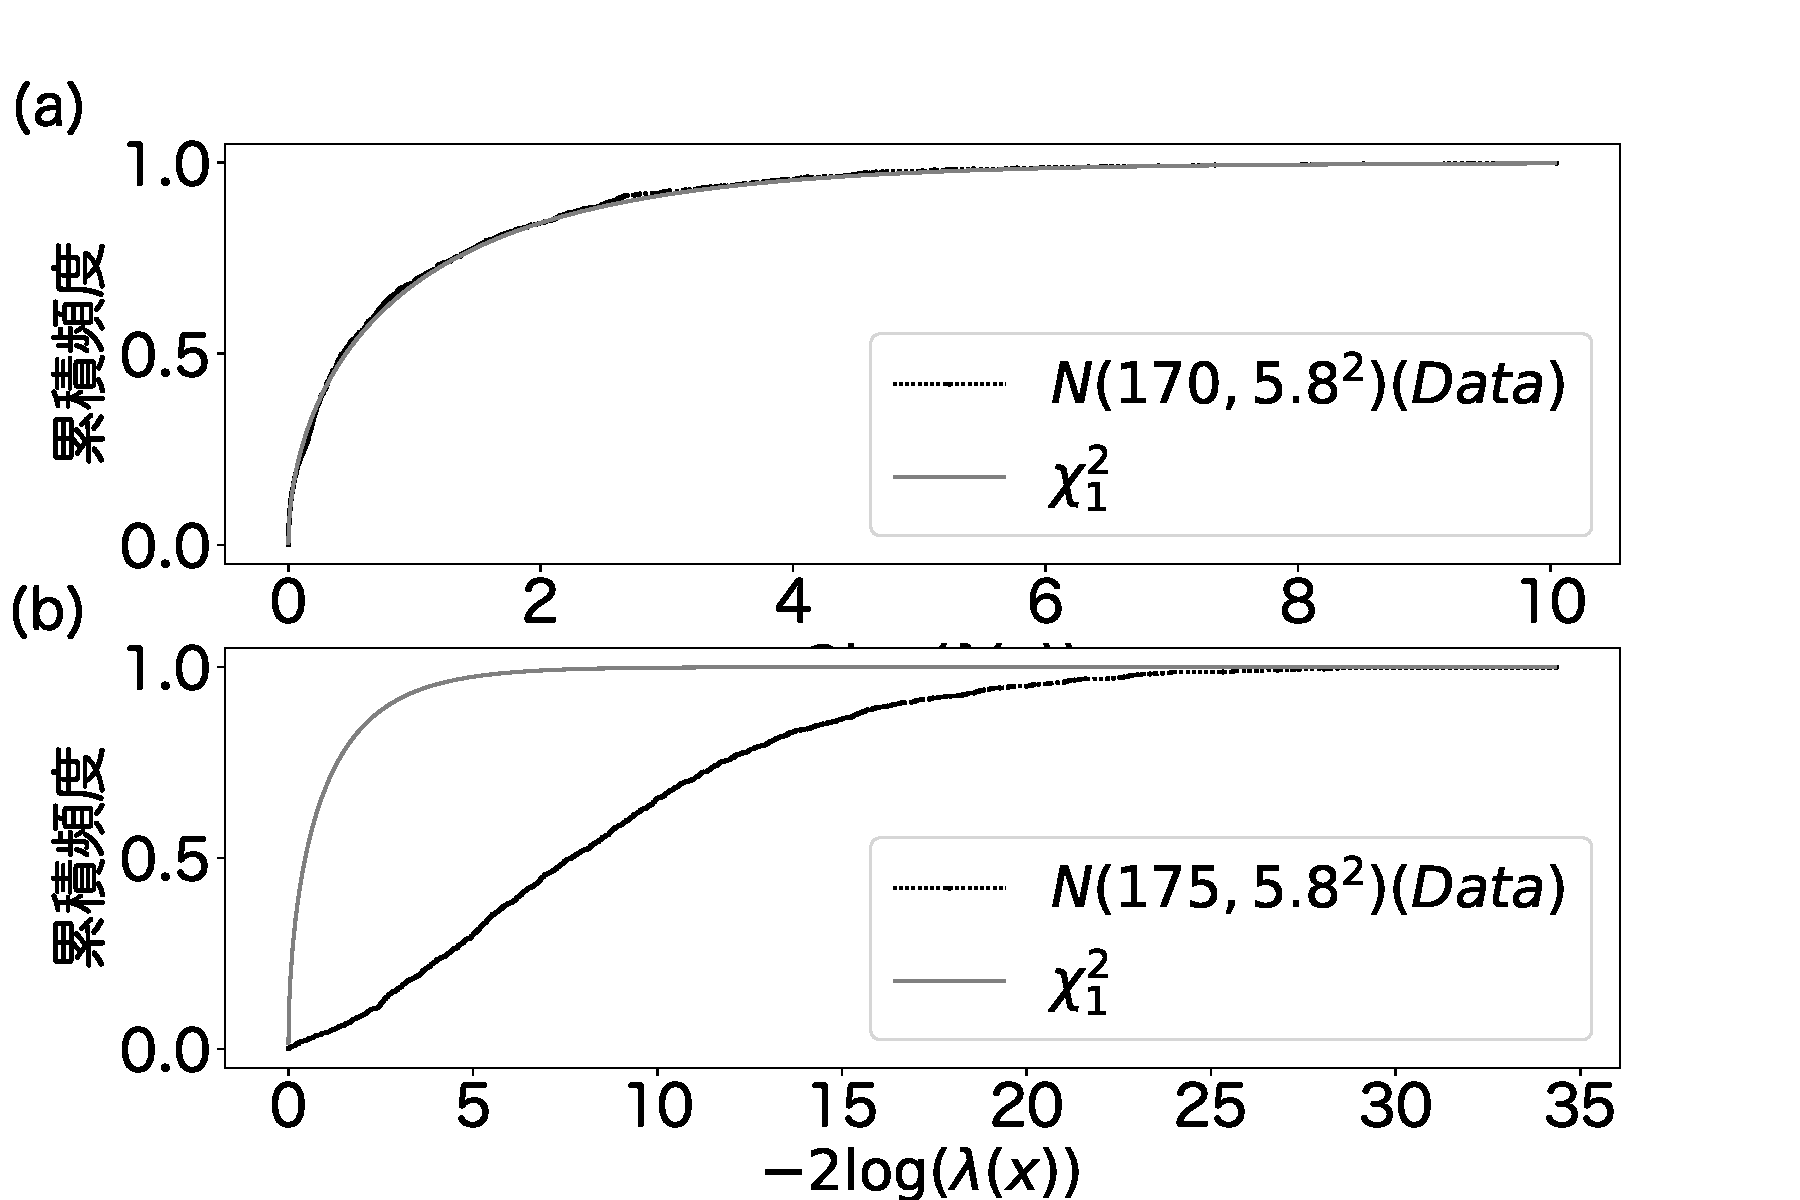
\includegraphics[width=15cm]{./image/04_/loglikeli_norm_test.pdf}
        \caption{対数尤度比の累積頻度。モデルは正規モデル$M(170;\sigma^2=5.8^2)$。(a)標本を$N(170,5.8^2)$からサンプリングした結果。(b)標本を$N(175,5.8^2)$からサンプリングした標本。}
        \label{fig:loglikelihood_test_simulation_norm}

      \end{center}
    \end{figure}

\subsection{データとモデルの乖離を検証する}
モデル上において、その標本を元にした最尤モデルにおける尤度比が$\chi^2_1$に従うことを示した。このことを元に、データをモデルによって予測可能かを調べる。手順は、
\begin{enumerate}
    \item 標本を$x$とする。
    \item モデル$M$における最尤推定量を計算する。
    \item モデル$M$および最尤モデル$M_{MLE}$における標本$x$に対する尤度を計算する
    \item 尤度比および$-2\log\lambda(x)$を計算し、$\chi^2_1$において珍しい値なのかを検証する。
\end{enumerate}
実際に、正規モデルにおいてこの手順をなぞってみる。
$M(\mu;\sigma^2)$における最尤モデルは、$M(\bar{x};\sigma^2)$である。
それぞれのモデルにおける尤度を計算し、$-2\log\lambda{x}$を計算すればよい。

\section{複雑なモデルでの尤度比検定}
次のモデル$M(\beta_1,\beta_2)$を考える。
\begin{enumerate}
    \item $x_i$は独立同分布
    \item $y_i$は以下に示す分布$p(y_i;\lambda_i)$に従う。
    \item $\lambda_i = \exp(\beta_1+\beta_2 x_i)$
    \item $y_i \sim p(y_i;\lambda_i) = \frac{\lambda_i^{y_i}\exp(-\lambda_i)}{y_i!}$
\end{enumerate}
無作為抽出した標本$x$における2つの最尤モデルを考える。
最初のモデルは、$\beta_2=0$とした上で、$\beta_2$に関する最尤推定を行なったモデル$M_1=M(\hat{\beta_1},\beta_2=0)$である。
このモデルでは、$x_i$に応じて、$\lambda_i$が変化しないので、$\lambda$が常に一定のモデルになる。言い換えれば、$y$が母数$\lambda=\exp(\beta_1)$のポアソン分布となるモデルである。
次のモデルは、$\beta_1,\beta_2$の両方について最尤推定を行なったモデル$M_2=M(\hat{\hat{\beta_1}},\hat{\hat{\beta_2}})$である。
このモデルにおいて、$(x_i,y_i)$はペアになっており、$x_i$に応じて$y_i$が揺らぎを持って決まる。

ここで、$M_1$における尤度比が$\chi_1^2$に従うことを確かめる。手順は以下の通りである。
\begin{enumerate}
    \item $M_1$においてサンプリングを行い、$(x_i,y_i)$からなる標本$X$を得る。$x_i$は、既存の標本$x$のものを使う。$(x_i,y_i)$に関してバラバラになった標本が得られる。
    \item $M_1$における標本$X$の尤度$L_1$を計算する。
    \item $M_2$における標本$X$の尤度$L_2$を計算する。
    \item $-2\log\frac{L_1}{L_2}$を計算する。以上を繰り返す。
\end{enumerate}
以上を行うと、$\chi^2_1$に従うことがわかる。図\ref{fig:loglikelihood_test_simulation_poisson}a,bに結果を載せている。
コードを書いておく。
\begin{lstlisting}
df  = pd.read_csv("https://raw.githubusercontent.com/tushuhei/statisticalDataModeling/master/data3a.csv")

def get_dd(d):
    d['y_rnd'] = np.random.poisson(np.mean(d.y),len(d.y))
    model1 = smf.glm(formula='y_rnd~1',data=d,
    family=sm.families.Poisson())
    model2 = smf.glm(formula = 'y_rnd~x',data=d,family=sm.families.Poisson())
    #print(fit1.summary())
    fit1 = model1.fit()
    fit2 = model2.fit()
    return fit1.deviance - fit2.deviance

l = []
for i in range(1000):
    l.append(get_dd(df))


x = sorted(l)
y = np.arange(len(l))/len(l)
plt.plot(x,y)
plt.plot(x, chi2.cdf(x,df = 1))
plt.show()
\end{lstlisting}


\begin{figure}
    \begin{center}
        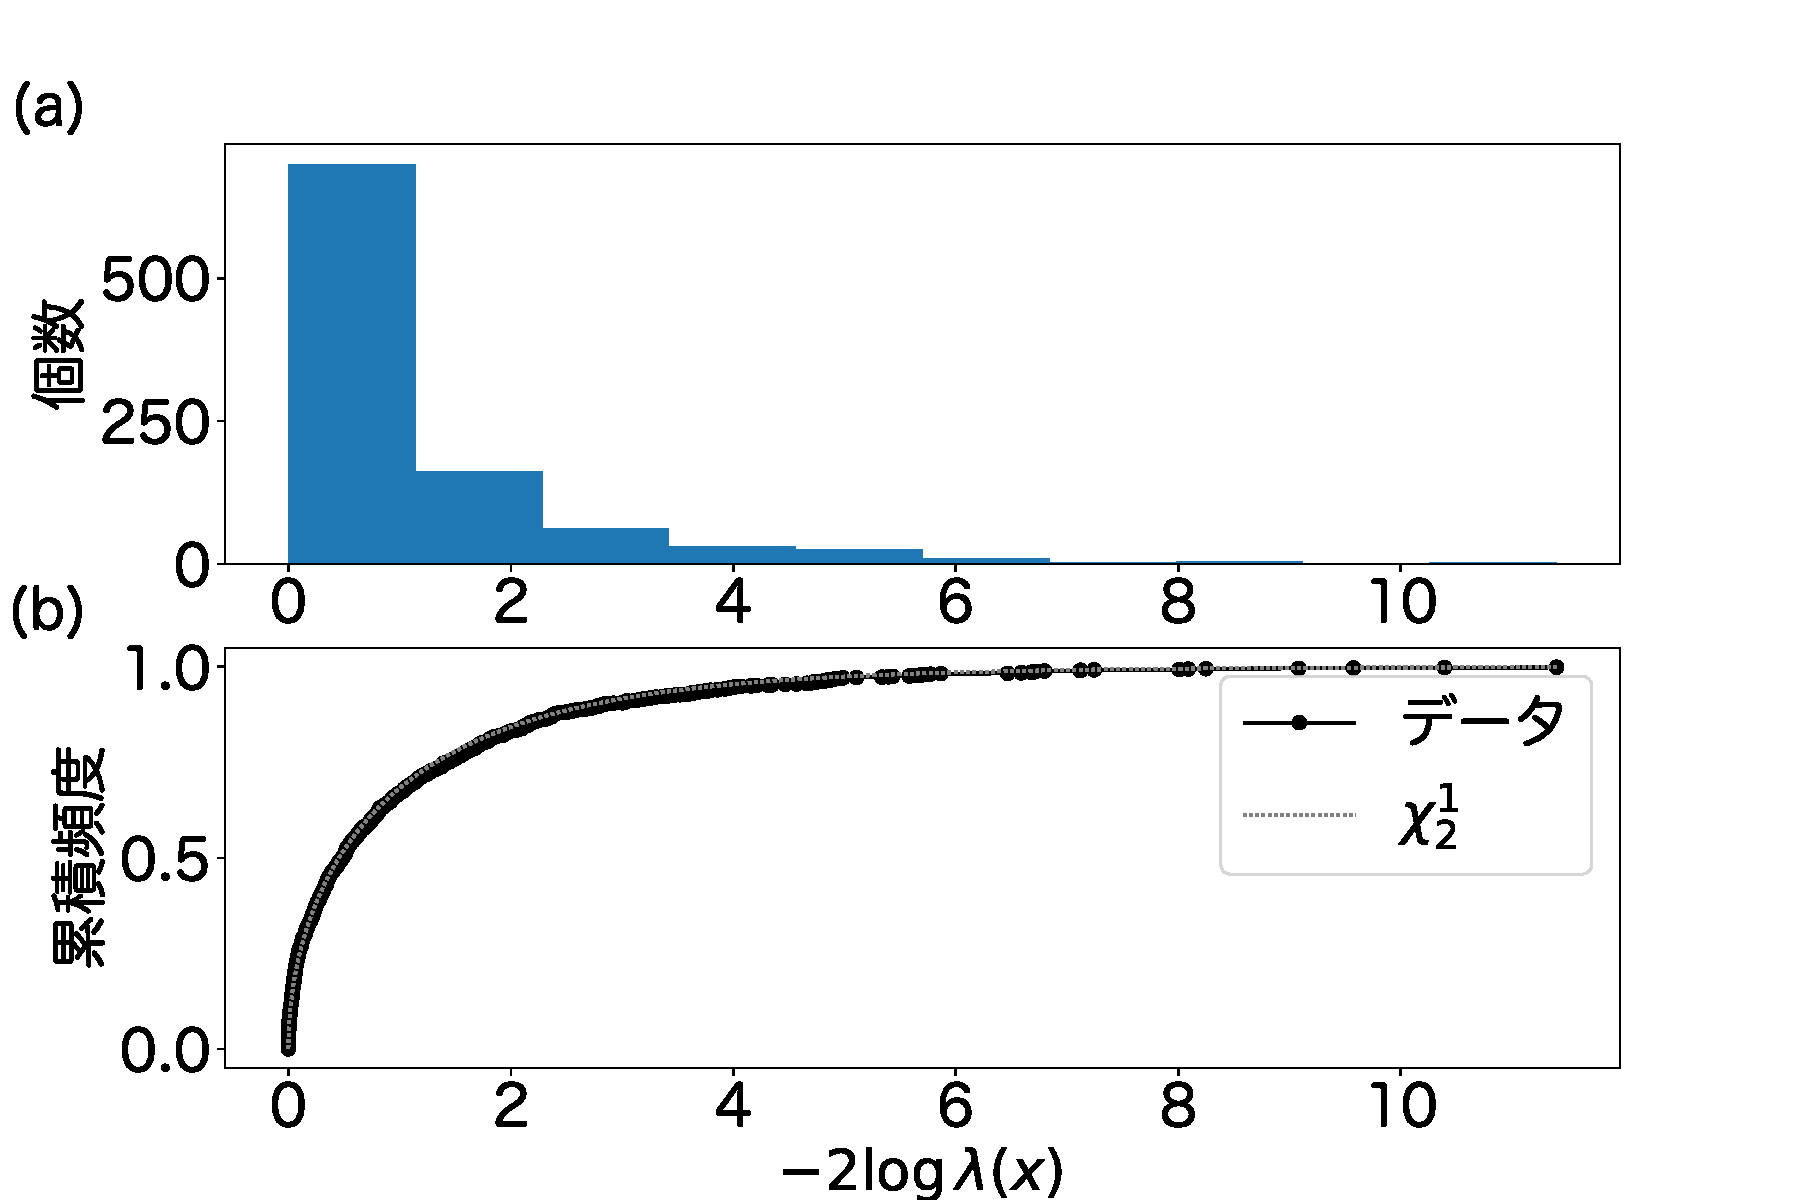
\includegraphics[width=15cm]{./image/04_/loglikeli_poisson_model_test.pdf}
        \caption{$M_1$における対数尤度比の累積頻度。(a)ヒストグラム(b)累積分布}
        \label{fig:loglikelihood_test_simulation_poisson}
    \end{center}
\end{figure}


データと、最尤モデル$M_1$との比較は同様に、
\begin{enumerate}
    \item 標本$x$の尤度$L_1$を$M_1$上で計算する。
    \item 標本$x$の尤度$L_2$を$M_2$上で計算する。
    \item $-2\log\frac{L_1}{L_2}$を計算する。
\end{enumerate}
最尤モデル$M_1$においてデータ$x$が予測できないなら、$-2\log\frac{L_1}{L_2}$が大きな値を取る。

最尤モデル$M_1$からサンプリングされた標本の尤度と、最尤モデル$M_2$での尤度を比較すると、$\chi^2_1$に従う。
なぜならば、ここにおける最尤モデル$M_2$のパラメータ$\beta_2$はほとんど0と変わりなく、小さな値をとるので、$M_1$と違いが少ない。
標本が$M_1$からサンプリングされていないなら、モデル$2$での最尤推定の結果、
$\beta_2$も$0$から離れてしまい、尤度比も大きくなるはずである。
$M_1$で標本$x$を予測しない方がよくないことを示す証拠の一つになる。
ただし、$M_2$が良い予測モデルであるのかは不明である。


$M_1$からサンプリングした標本で、$M_1$および$M_2$を推定したモデルの尤度比は$\chi^2_1$に従う。
実際の標本を元に、$M_1,M_2$を推定し、そのモデルの尤度比は、$M_1$による予測ができるならば、$\chi^2_1$程度だと考えられる。
実際にこの例では、尤度比が大きくなり、$\chi^2_1$においては珍しい値になったので、
$M_1$により予測しない方が良さそうと言う根拠の一つになりうる。
$M_2$の$\hat\hat\beta_2$のパラメータがどうなっているかなども気にした方が良さそう。







